\documentclass[a4paper,10pt]{article}
\usepackage[utf8]{inputenc}
\usepackage{enumerate}
\usepackage{amsmath}
\usepackage{graphicx}
\usepackage{listings}
\usepackage{float}
\usepackage[caption = false]{subfig}
\usepackage[parfill]{parskip}
\usepackage{url}

\title{Project 2: modelling a star}
\author{Christer Dreierstad\footnote{I have been working together with Hans Erlend Bakken Glad.}}
\date{29.04.2018}

\begin{document}
\maketitle
\section{Introduction}
Expanding on our previous model of a stellar core require us to consider another form of energy transport; convection. By comparing a pocket of gas rising inside the solar atmosphere 
with its surroundings, we apply a method to decide whether the gas in unstable or not. The rise is fast enough so that no energy is exchanged, but slow enough so that there can be pressure equilibrium with the surroundings. There are now two scenarios to consider, either the pocket will be in total equilibrium with its surroundings (an adiabatic expansion), or there could be a difference in the density. A difference in density means the pocket will be buoyant and a buoyancy force will act upon it, resulting in the pocket moving. If the density differs throughout, the gas is unstable and energy will be transported by movement; convective energy transport. By making a model that looks at the different temperature gradients of the star, we can model the energy transport throughout the star. At the end we find a model that has radiative zone reaching $\approx 15$\% out, radiation outside the core reaching out towards the convective zone outside the core, which covers $\approx 25$\% of the top of the solar atmosphere. The final model has an end mass of $4.4\%$, end luminosity of $0.1\%$ and an end radius of $0.026\%$ of its respective initial values. 


\section{Model}
We consider four different temperature gradients, $\nabla^*$ - for the star, $\nabla_{stable}$ - temperature gradient needed for all the energy to be transported by radiation (no convection), $\nabla_p$ - for the pocket and $\nabla_{ad}$, which is the temperature gradient if the expansion of the pocket is adiabatic. 

\subsection{Instability criterion} A criterion for instability is that the temperature gradient for the pocket is larger than for an adiabatic expansion of the pocket, this is because $\nabla_p$ then must satisfy a larger transfer of energy flux. Also $\nabla_{ad}$ must be smaller, since the pocket then cools by both adiabatic expansion and radiation. So our first instability criterion is that $\nabla_p > \nabla_{ad}$ if the gas is unstable. We can also see from the equation of convective flux, equation \eqref{eq:Fc}, that $\nabla^* > \nabla_p$ in order for there to be convective flux with real values. Also from equation (5.73), regarding the buoyancy force, in the notes, $\nabla^* > \nabla_p$ for the buoyancy force to be positive so that the pocket moves upwards to the surface. So our second instability criterion is that $\nabla^* > \nabla_p$. Since $\nabla_{stable}$ is the temperature gradient needed for the gas to be stable, a requirement for the gas to be unstable is simply that $\nabla_{stable} > \nabla^*$ because there is less energy transported by radiation. To sum up, we have the following criteria for the gas to be unstable: $\nabla_{stable} > \nabla^* > \nabla_p > \nabla_{ad}$. The instability criterion for our numerical model is $\nabla_{stable} > \nabla_{ad}$.


We now aim to find the difference of the temperature gradients for the star and the parcel (i.e. $(\nabla^* - \nabla_p)$) as a function of known parameters.

\subsection{Analytical}
The energy transport is related to the energy flux. We have from the notes equations for both convective and radiative flux given as
%
\begin{align}\label{eq:Fc}
F_C &= \rho c_P T \sqrt{g\delta}H_P^{-3/2}\bigg(\frac{l_m}{2}\bigg)^2(\nabla^* - \nabla_p)^{3/2} \\
F_R &= \frac{16\sigma T^4}{3\kappa \rho H_P}\nabla^*,\label{eq:Fr}
\end{align}
%
where $H_P$ is the pressure scale height, $l_m$ is the mixing length and $\delta = -(\partial \ln P/\partial \ln T)$. The pressure scale height we know to be $H_P = -P\frac{\partial r}{\partial P}$, to find what it is we use that for an ideal gas we have
%
\begin{align*}
\frac{dr}{dP} = -\rho g \Leftrightarrow \rho = -\frac{1}{g}\frac{dP}{dr},
\end{align*}
%
where g is the gravitational acceleration of the star given by $g = Gm(r)/r^2$, where G is the universal gravitational constant. For an ideal gas we know from the last model that 
%
\begin{align}\label{eq:P_to_Hp}
P = \frac{k_B T}{m_u \mu} \rho = \frac{k_B T}{m_u \mu} \bigg(-\frac{1}{g}\frac{dP}{dr}\bigg)
\Rightarrow -P\frac{dr}{dP} = \frac{k_B T}{m_u \mu g} = H_P.
\end{align}
%
The mixing length $l_m = \alpha H_P$ for some arbitrary constant $\alpha$ between $0.5$ and $2$. To find $\delta$ for an ideal gas, we can use the expression the pressure in equation \eqref{eq:P_to_Hp}. We further integrate by parts so that $\delta = \frac{T}{P}\frac{\partial P}{\partial T}$. Performing the partial derivative of P with respect to T yields $P' = P/T$, so $\delta = \frac{T}{P}\frac{P}{T} = 1$ for an ideal gas. Further we have the sum of convective and radiative flux given as
%
\begin{align}\label{eq:Fc+Fr}
F_R + F_C = \frac{16\sigma T^4}{3\kappa \rho H_P}\nabla_{stable}.
\end{align}

We now add equations \eqref{eq:Fc} and \eqref{eq:Fr} and set them equal to \eqref{eq:Fc+Fr}, and solve the equation for $(\nabla^* - \nabla_p)^{3/2}$ which we substitute to $\xi^3$:
%
\begin{align*}
\frac{16\sigma T^4}{3\kappa \rho H_P}\nabla^* + \rho c_P T \sqrt{g\delta}H_P^{-3/2}\bigg(\frac{l_m}{2}\bigg)^2(\nabla^* - \nabla_p)^{3/2} = \frac{16\sigma T^4}{3\kappa \rho H_P}\nabla_{stable},
\end{align*}
%
we gather $16\sigma T^4/3\kappa \rho H_P$ outside a parenthesis containing $\nabla_{stable} - \nabla^*$ and solve the equation as mentioned above
%
\begin{align}
\xi^3 &= \frac{16\sigma T^4(\nabla_{stable} - \nabla^*)/3\kappa \rho H_P}{\rho c_P T \sqrt{g\delta}H_P^{-3/2}\big(\frac{l_m}{2}\big)^2}(\nabla_{stable} - \nabla^*) \\
&= \frac{64 \sigma T^3}{3\kappa \rho^2 c_P l_m^2}\sqrt{\frac{H_P}{g\delta}}(\nabla_{stable} - \nabla^*)\\
&= \frac{U}{l_m^2}(\nabla_{stable} - \nabla^*) \label{eq:ksi^3}
\end{align}

From equation (5.73) in the notes we have an expression for the difference of the temperature gradient of the pocket and the temperature gradient of it if the expansion was adiabatic. We consider adding and subtracting the temperature gradient of the star such that $(\nabla_p - \nabla_{ad}) = (\nabla^* - \nabla_{ad}) - (\nabla^* - \nabla_p)$, where we insert equation (5.73) on the left hand side
%
\begin{align}\label{eq:5.12_1}
\frac{32\sigma T^3}{3\kappa \rho^2 c_P}\sqrt{\frac{4H_P}{g\delta l_m^3}}(\nabla^* - \nabla_p)^{1/2} \frac{S}{Qd} = (\nabla^* - \nabla_{ad} )-(\nabla^* - \nabla_p),
\end{align}
%
where we have inserted equation (5.78) from the notes for the velocity in (5.73). The factor $S/Qd$ is a geometrical factor of the pocket, $S = 4\pi r_p^2$ is the surface area, $Q = \pi r_p^2$ is the surface normal to the velocity and $d = 2r_p$ is the diameter of the pocket. We are considering that the pocket moves $\delta r = l_m/2$, and we set the radius to be the same, this yields $S/Qd = 4/l_m$. Returning to equation \eqref{eq:5.12_1} with substitution $U = (64\sigma T^3/3\kappa \rho^2 c_P )\sqrt{H_P/g\delta}$ 
%
\begin{align*}
\frac{4U}{l_m}(\nabla^* - \nabla_p)^{1/2} + (\nabla^* - \nabla_p) - (\nabla^* - \nabla_{ad}) = 0,
\end{align*}
%
which by the substitution for $\xi$ yields a second order polynomial with respect to the difference of the temperature gradient of the star and the parcel $\xi$:
%
\begin{align}
\xi^2 + \frac{4U}{l_m}\xi - (\nabla^* - \nabla_{ad}) = 0.
\end{align}
%
Solving this equation gives that $\xi = \pm \frac{1}{2}\sqrt{(4U/l_m)^2 + 4(\nabla^* - \nabla_{ad})} - 2U/l_m$. We discard the solution for the negative sign, since that would mean the temperature gradient of the parcel was larger than the one of the star. We now solve the expression for $\xi$ found above for $\nabla^*$:
%
\begin{align*}
\bigg(2\xi + \frac{4U}{l_m}\bigg)^2 &= \bigg(\frac{4U}{l_m}\bigg)^2 + 4(\nabla^* - \nabla_{ad})\\
4\xi^2 + 4\xi \frac{4U}{l_m} + \bigg(\frac{4U}{l_m}\bigg)^2 &= \bigg(\frac{4U}{l_m}\bigg)^2 + 4(\nabla^* - \nabla_{ad}).
\end{align*}
%
Solving for $\nabla^*$ yeilds
%
\begin{align}\label{eq:nab*}
\nabla^* &= \xi^2 + \xi\frac{4U}{l_m} + \nabla_{ad},
\end{align}
%
which inserted into equation \eqref{eq:ksi^3} yields a third order equation:
%
\begin{align*}
\xi^3 = \frac{U}{l_m^2}(\nabla_{stable} - \xi^2 - \xi\frac{4U}{l_m} - \nabla_{ad}),
\end{align*}
%
resulting in
\begin{align}
\frac{l_m^2}{U}\xi^3 + \xi^2 + \xi\frac{4U}{l_m} - (\nabla_{stable} - \nabla_{ad}) = 0
\end{align}
%

To find an equation for $\nabla_{stable}$ we consider the equation for the total flux $F = L/4\pi r^2 = F_R + F_C$, where $F_R + F_C$ is given by equation \eqref{eq:Fc+Fr}. We then get
%
\begin{align*}
\frac{L}{4\pi r^2} = \frac{16\sigma T^4}{3\kappa \rho H_P}\nabla_{stable},
\end{align*}
%
which we solve for $\nabla_{stable}$ yielding
%
\begin{align}\label{nab_stab}
\nabla_{stable} = \frac{3\kappa \rho LH_P}{64\pi \sigma r^2 T^4}.
\end{align}
%
$\nabla_{ad}$ is given by equation (5.44) in the notes:
%
\begin{align}\label{eq:nab_ad}
\nabla_{ad} = \frac{P\delta}{T\rho c_P}.
\end{align}
%

\subsection{Numerical}
When evaluating the parameters of the stars we now have to check whether there is convection in the gas or not. We have the instability criterion from previous $\nabla_{stable} > \nabla_{ad}$. For each mass shell we calculate inwards, we calculate to find $\xi$ by a quadratic solver, and make sure we collect the real valued solution. There are both positive and negative roots produces by this method, and while we are only interested in the positive values, we discard the solution in our model when considering the instability criterion. If the instability criterion is fulfilled, we need a new temperature gradient for the gas. By manipulating $\nabla^*$ we can produce a new $dT/dm$. We have that 
%
\begin{align*}
\nabla^* = \frac{\partial T}{\partial P} = \frac{P}{T}\frac{\partial T}{\partial P}.
\end{align*}
%
If we multiply the aforementioned equation by $(T/P) \partial P/\partial m$ we get
%
\begin{align}\label{eq:nab->dTdm}
\frac{T}{P}\nabla^* \frac{dP}{dm} = \frac{T}{P}\frac{P}{T}\frac{\partial T}{\partial P}\frac{\partial P}{\partial m} = \frac{dT}{dm}.
\end{align}
%
If the instability criterion is not fulfilled, we return to the model presented the previous paper to calculate the next $dT/dm$. At the same time we update $\nabla^*$ using the aforementioned $dT/dm$ by the same method presented in equation \eqref{eq:nab->dTdm} so that
%
\begin{align}
\nabla^* = \frac{P}{T}\frac{1}{dP/dm}\frac{dT}{dm} = \frac{P}{T}\frac{dT}{dP} = \frac{d\ln T}{d\ln P}.
\end{align}
%

\subsection{Finding the best model}
Creating a realistic model we have to make sure that the mass, radius and luminosity goes towards zero at the same time. Thinking back to the previous paper, we reduced the initial radius and density by respectively $54.3\%$ $63\%$, while increasing the initial temperature by $50\%$. We now take a look at the instability criterion to see what we can expect when changing the initial values for radius, density and temperature individually, while keeping the other initial values constant.

\subsubsection{Radius}
When varying the radius, we would expect that for smaller radii the temperature gradient across the star would increase, and dominate at the core. Looking at equations \eqref{nab_stab} and \eqref{eq:nab_ad} we see that $\nabla_{stable} \propto 1/r^2$, one would therefore expect the convection to become greater as the radius is reduced, but the overall temperature will dominate in equation \eqref{nab_stab}, making it smaller. We see in figure \ref{fig:r_vary} that increasing the temperature will reduce the radiative energy transport in the core, while increasing the convective energy transport outside the core. Further we observe that the convective instability seem to be reduced as the radius increases.

\begin{figure}[H]
\centering
\subfloat[Initial radius times 0.2.]{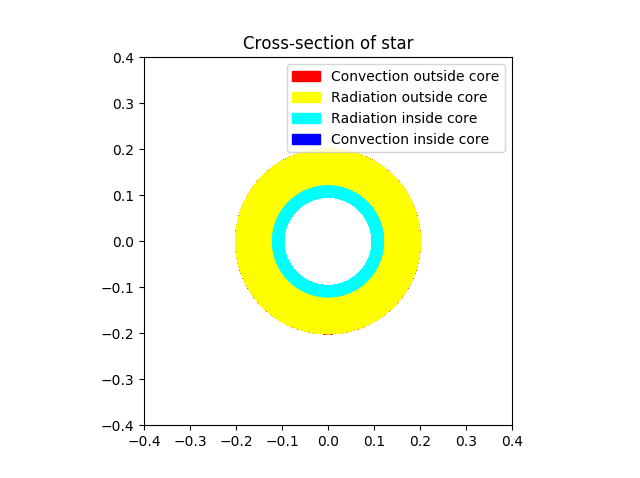
\includegraphics[width = 4cm]{r02.png}}
\subfloat[Initial radius times 0.75.]{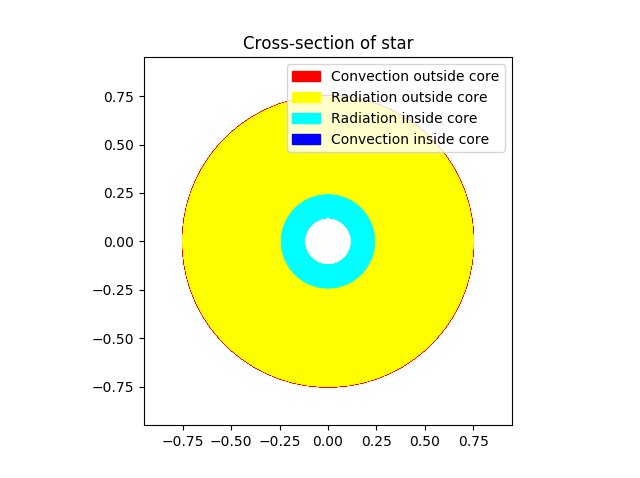
\includegraphics[width = 4cm]{r075.png}}
\subfloat[Initial radius.]{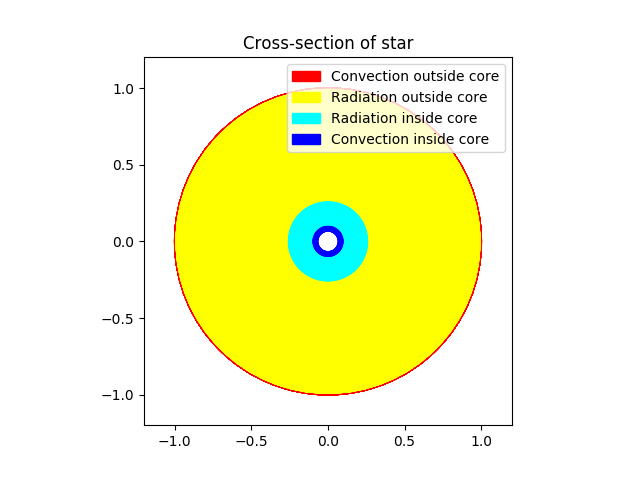
\includegraphics[width = 4cm]{r1.png}} \\
\subfloat[Initial radius times 2.]{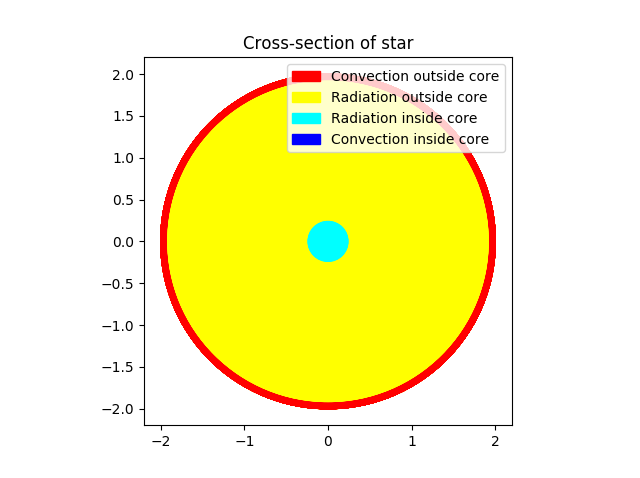
\includegraphics[width = 4cm]{r2.png}}
\subfloat[Initial radius times 3.5.]{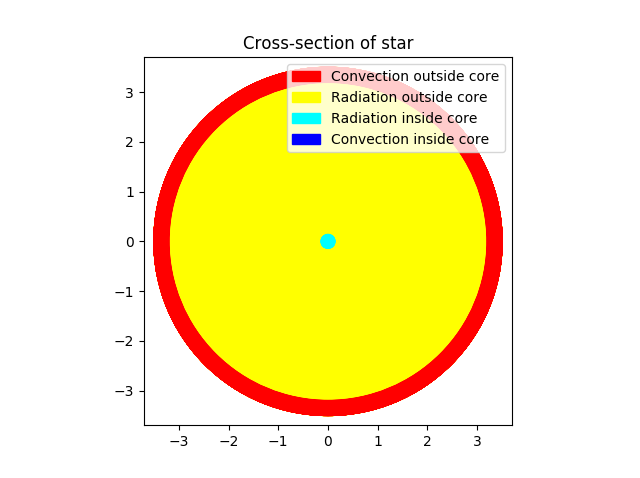
\includegraphics[width = 4cm]{r35.png}}
\subfloat[Initial radius times 5.]{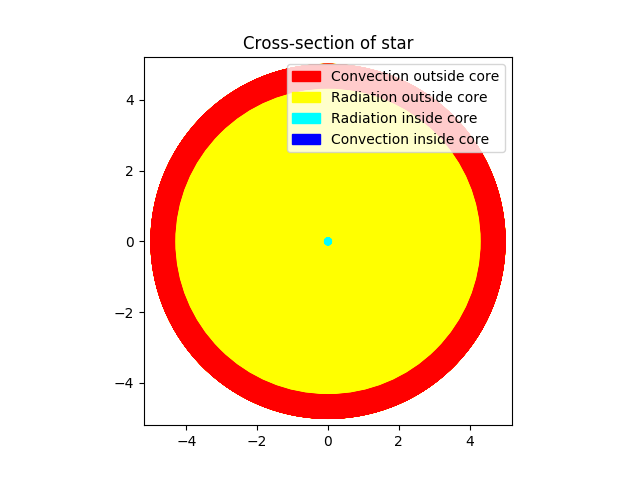
\includegraphics[width = 4cm]{r5.png}}
\caption{Cross section of the star with initial radius multiplied by factors ranging from 0.2 to 5. The other initial conditions are held at initial value.}
\label{fig:r_vary}
\end{figure}


\subsubsection{Density}
By equations \eqref{nab_stab} and \eqref{eq:nab_ad} we see, when only varying the density, that $\nabla_{stable} \propto \rho > \nabla_{ad} \propto 1/\rho$. We therefore expect that we should get convection if $\rho^2 > 1$. In figure \ref{fig:rho_vary} we see that the convective zone outside the core grows larger as the density increases. We also observe that the convective instability increase with the density.


\begin{figure}[H]
\centering
\subfloat[Initial density times 0.7.]{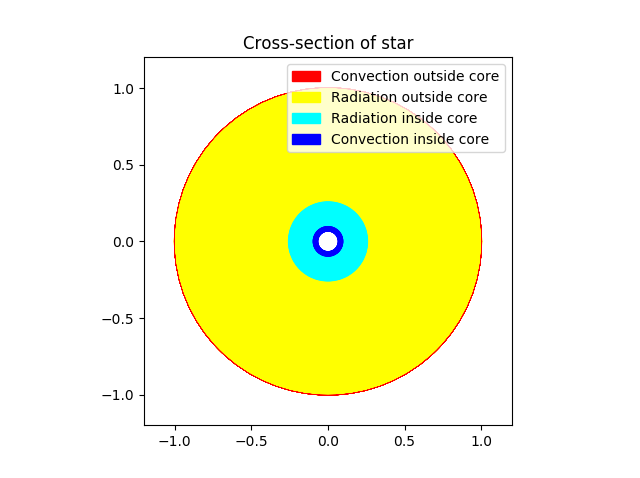
\includegraphics[width = 4cm]{rho07.png}}
\subfloat[Initial density.]{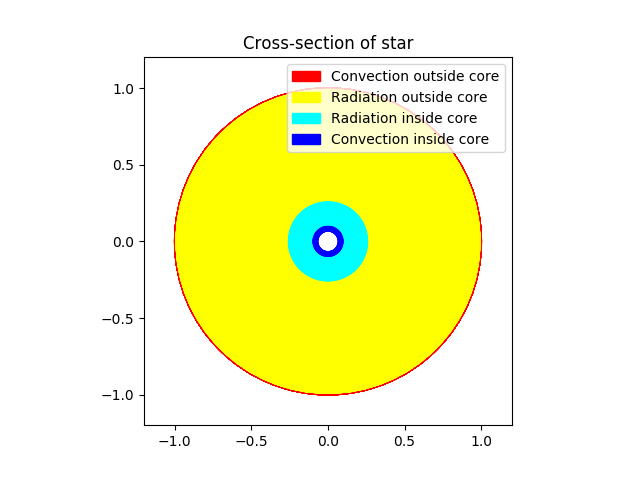
\includegraphics[width = 4cm]{rho1.png}}
\subfloat[Initial density times 15.]{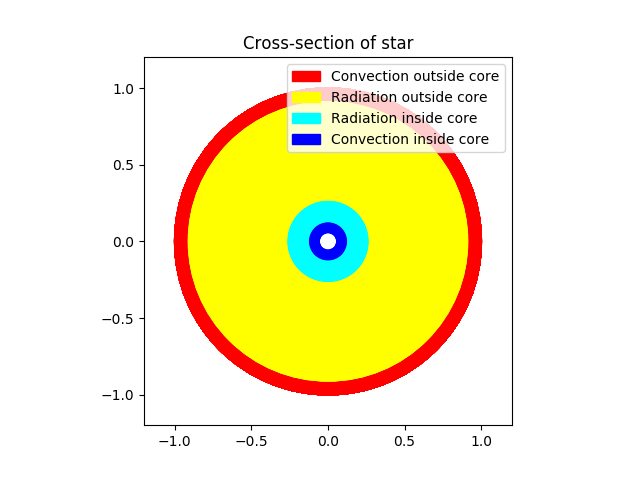
\includegraphics[width = 4cm]{rho15.png}} \\
\subfloat[Initial density times 30.]{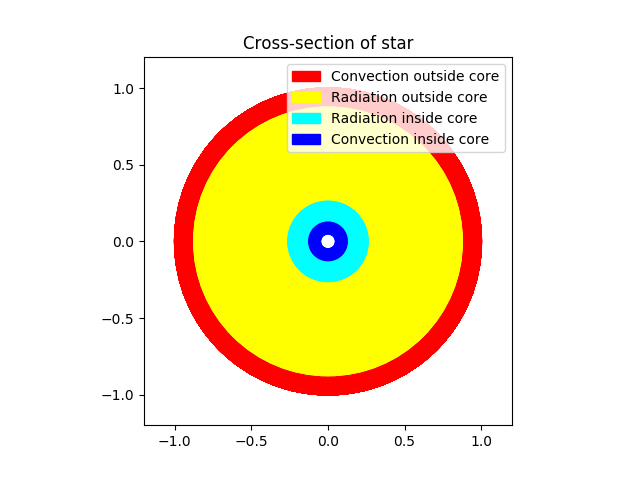
\includegraphics[width = 4cm]{rho30.png}}
\subfloat[Initial density times 50.]{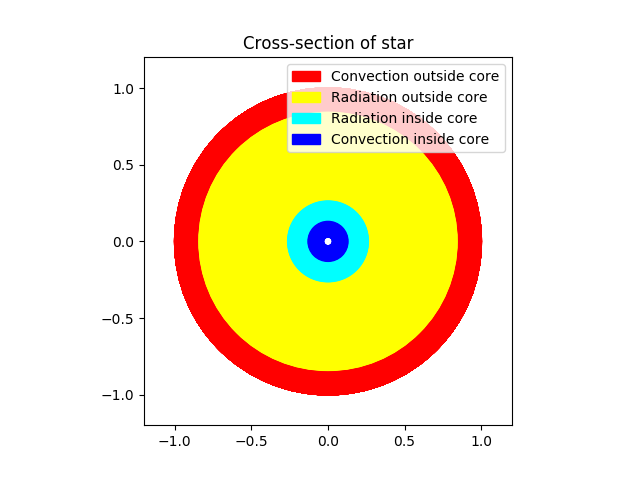
\includegraphics[width = 4cm]{rho50.png}}
\subfloat[Initial density times 70.]{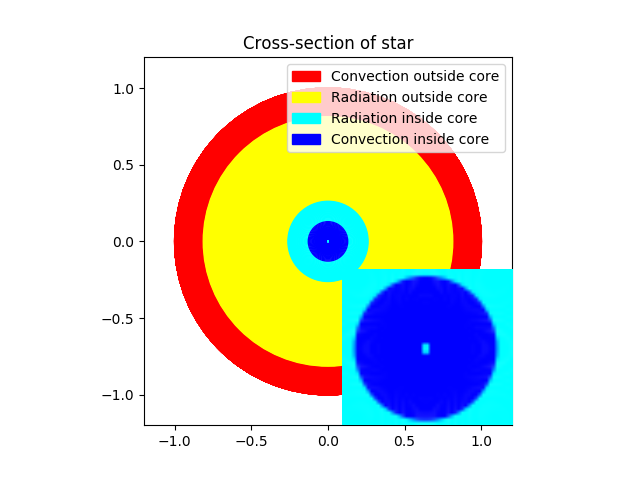
\includegraphics[width = 4cm]{rho70.png}}
\caption{Cross section of the star with initial density multiplied by factors ranging from 0.9 to 70. The other initial conditions are held at initial value.}
\label{fig:rho_vary}
\end{figure}

\subsection{Temperature}
By equations \eqref{nab_stab} and \eqref{eq:nab_ad} we see, when only varying the temperature, that $\nabla_{stable} \propto 1/T^4 > \nabla_{ad} \propto 1/T$. We therefore expect convection if $T^3 < 1$. In figure \eqref{fig:T_vary} we can see that our model behaves as we expect. We observe that varying the temperature seems to only have an effect on the outer convective zone, and that the core remains convectively unstable.

\begin{figure}[H]
\centering
\subfloat[Initial temperature times 0.9.]{\includegraphics[width = 6cm]{T09.png}}
\subfloat[Initial temperature times 0.9.]{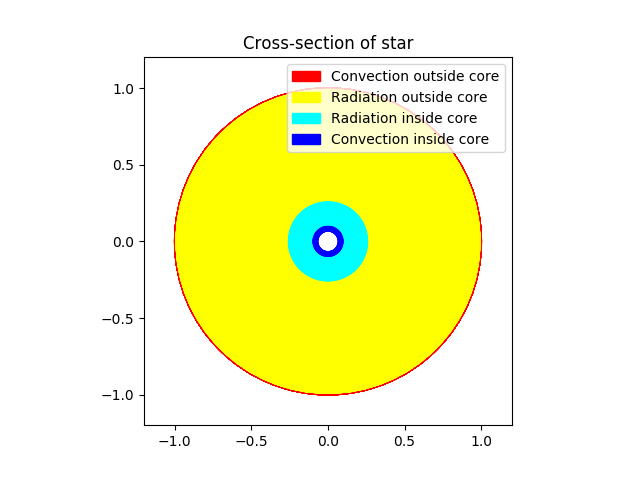
\includegraphics[width = 6cm]{T1.png}} \\
\subfloat[Initial temperature times 3.]{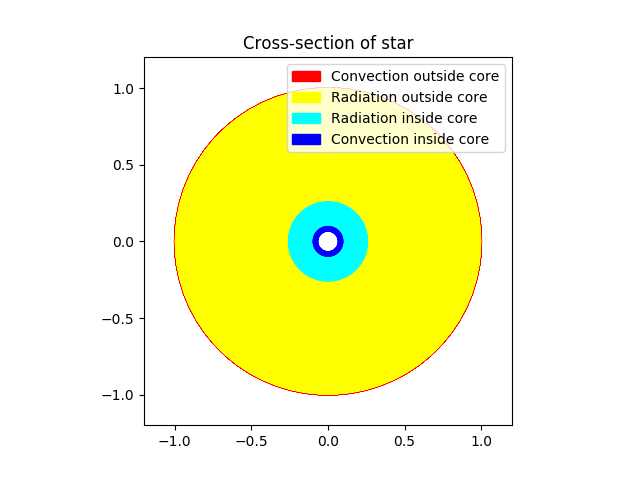
\includegraphics[width = 6cm]{T3.png}} 
\subfloat[Initial temperature times 5.]{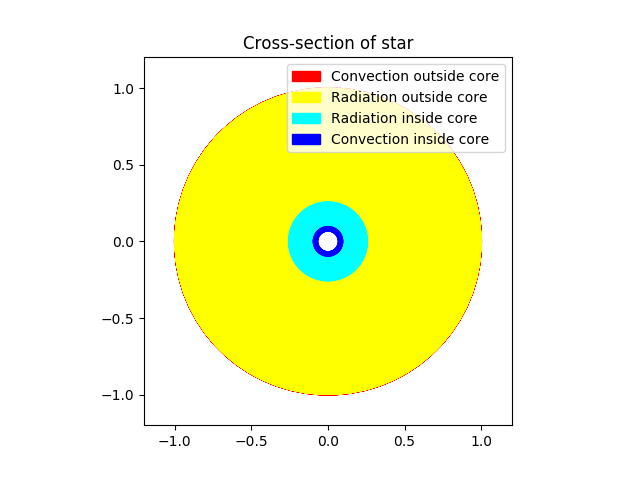
\includegraphics[width = 6cm]{T5.png}}
\caption{Cross section of the star with initial temperature multiplied by factors ranging from 0.9 to 5. The other initial conditions are held at initial value.}
\label{fig:T_vary}
\end{figure}

\subsection{Splitting energy production}
Since the PPIII $\approx 0$, we choose to ignore it in the calculations. When splitting the energy production we consider the rate of $r_{pp}$ decided by $r_{33}/(r_{33} + r_{34})$ and $r_{34}/(r_{33} + r_{34})$, summed up this is approximately 1. The fraction of the total reaction rates for PPI and PPII are found by the two equation above. We can then find the respective energy production by 
\begin{align*}
\epsilon_{PPI} = \epsilon_{r_{pp}} \frac{r_{33}}{r_{33} + r_{34}} + \epsilon_{r_{33}}, 	\epsilon_{PPII} = \epsilon_{r_{pp}} \frac{r_{34}}{r_{33} + r_{34}} + \epsilon_{r_{34}} + \epsilon_{r_{7e}} + \epsilon_{r_{71'}} 
\end{align*}
%
\section{Results}
\subsection{Varying initial condition based on the model found in previous paper}
When varying the initial condition trying to find a model that has the radius, luminosity and mass going to 0 together, we started with inspiration from the values found in the previous paper, to see how the star behaved. Reducing the density proved to have no success when trying to get a convective zone outside the core. Further there were problems having the luminosity and radius simultaneously go to 0 at the same time. We did not succeed in getting the radius below 8\%. The model often proved nonphysical, where the pressure, density and temperature seemed to become stable at the core, as the plots flattened. The temperature was also more linear than one can see in figure \ref{fig:r_plots}(e). We expect the pressure, density and temperature to rise as the radius becomes smaller. Basing the method of finding best fit values on the values found in the previous paper therefore proved unsuccessful.

\subsection{Varying initial conditions based instability criterion}
Based on the plots presented by figures \ref{fig:r_vary}, \ref{fig:rho_vary} and \ref{fig:T_vary} we decided to start with increasing the density by 50, increase the radius somewhere in the interval 1-2 while reducing the temperature slightly. We did not need to change the density further. Changing the radius below 1.5 times the initial value produced a convectively unstable core. Increasing the radius more than 1.5 resulted in a reduced size of the radiative zone in the core, while increasing the convective zone outside the core. Increasing above 1.5 also resulted in issues with the end mass not going below 5\% of the initial value. The final cross section is found in figure \ref{fig:cross}(a). When comparing the cross section of the final model with the cross section of the sun found in figure \ref{fig:cross}(b) we see that there are clear similarities regarding the thickness of the outer convective zone, the outer radiative zone and the core.

\begin{figure}[H]
\centering
\subfloat[]{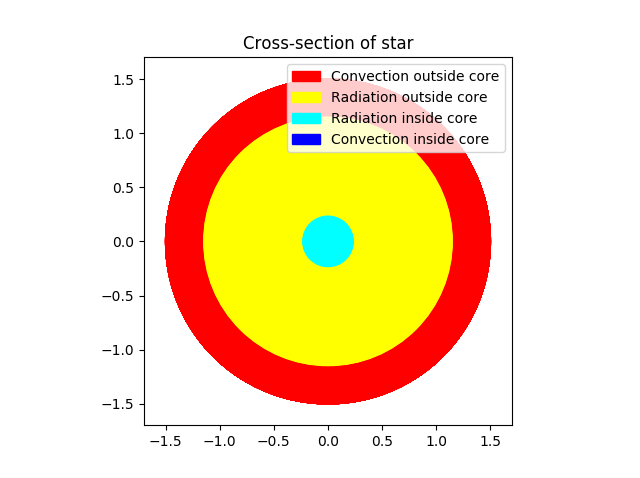
\includegraphics[width = 6cm]{cross.png}}
\subfloat[]{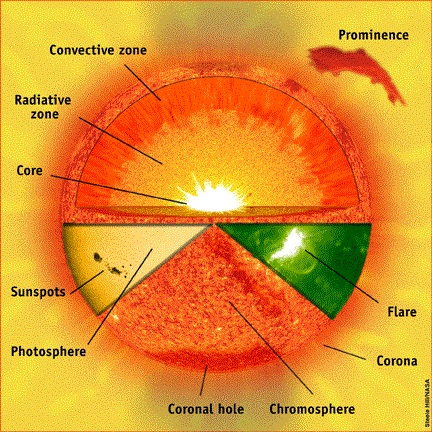
\includegraphics[width = 6cm]{layers.jpg}}
\caption{}
\label{fig:cross}
\end{figure}

\subsection{Figures}
In figure \ref{fig:r_plots} we can see in (a) that the luminosity is below 0.995 reaching out more than 10\% of the initial radius. The plots looks like we would expect, the density, pressure and temperature increase rapidly as we approach the core and the temperature behaves exponential.
%
In figure \ref{fig:nab_eps}(a) we can see that there is convection close to the surface of the star. In (b) we see that the energy production happens in the core, as we would expect, and that the energy production is PP2 dominated for low radii, where the temperature is high and PP2 and PP3 dominated for large radii, where the temperature is low. In (c) we see that the flux matches what we have summed up so far; convective flux at the outer solar atmosphere, and radiative flux going inward.

\begin{figure}[!]
\centering
\subfloat[Relative luminosity.]{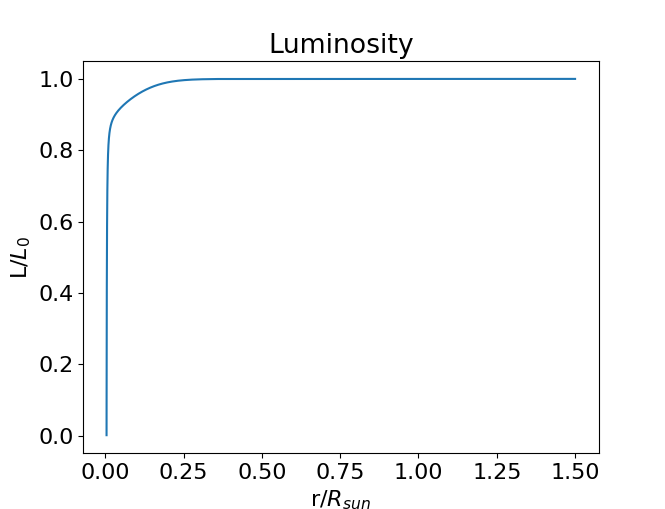
\includegraphics[width = 6cm]{L.png}}
\subfloat[Relative mass.]{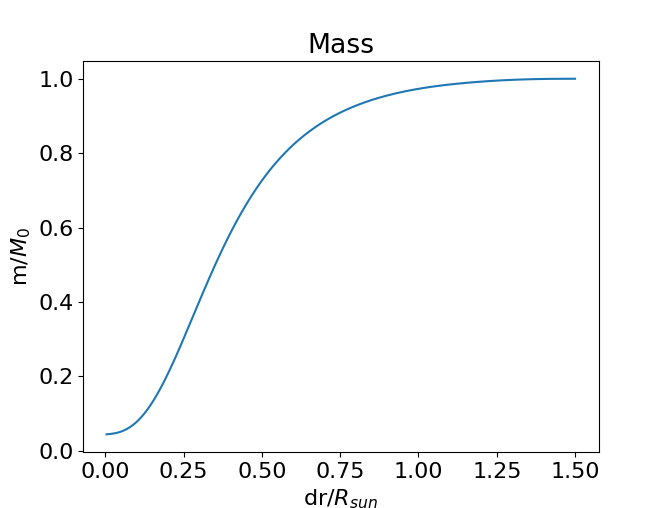
\includegraphics[width = 6cm]{m.png}} \\
\subfloat[Relative logarithmic pressure.]{\includegraphics[width = 6cm]{P.png}} 
\subfloat[Relative logarithmic density.]{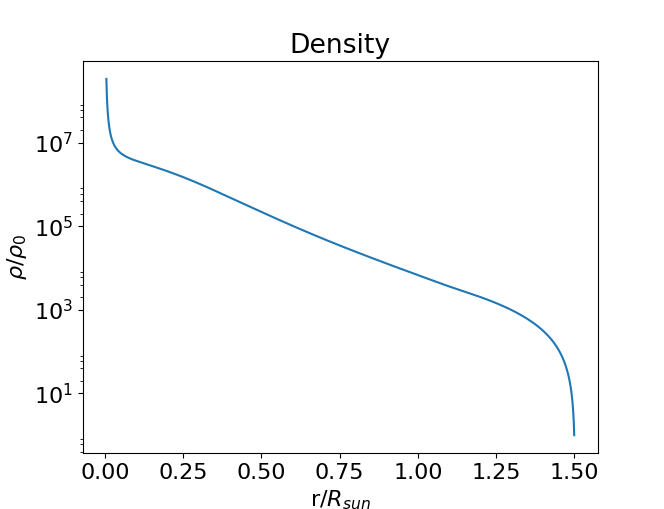
\includegraphics[width = 6cm]{rho.png}} \\
\subfloat[Relative temperature.]{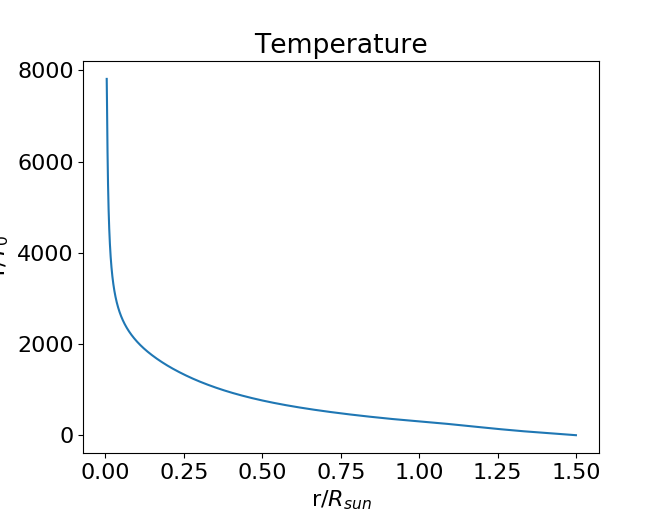
\includegraphics[width = 6cm]{T.png}}
\subfloat[Cross section for sanity check (no more room elsewhere).]{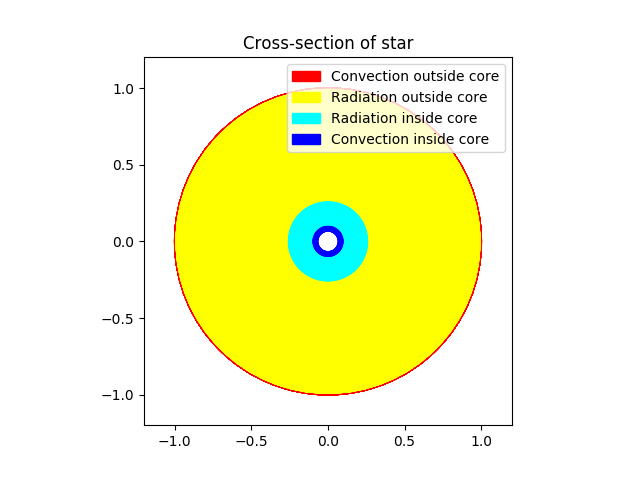
\includegraphics[width = 6cm]{cross_sanity.png}}
\caption{From subfigures (a)-(e) we find the respective values as functions of radius relative to the radius of the sun.}
\label{fig:r_plots}
\end{figure}

\begin{figure}[H]
\centering
\subfloat[Logarithmic temperature gradient as a function of radius.]{\includegraphics[width = 6cm]{nab.png}}
\subfloat[Relative energy as a function of radius.]{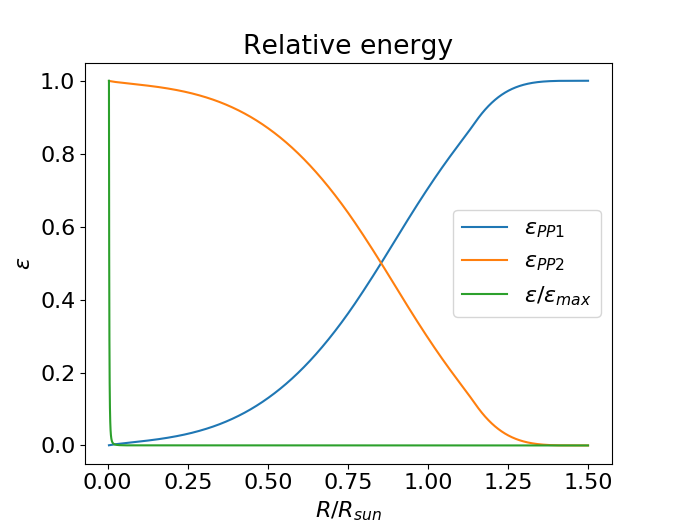
\includegraphics[width = 6cm]{eps.png}}\\
\subfloat[Relative flux as a function of the radius.]{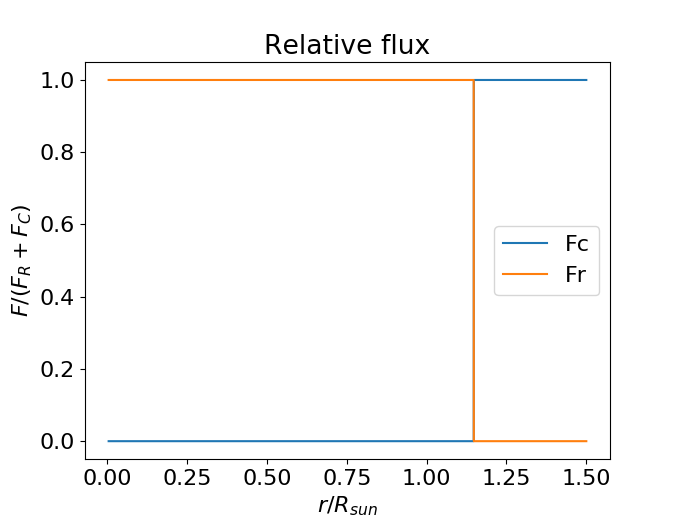
\includegraphics[width = 6cm]{Flux.png}}
\subfloat[Sanity check for temperature gradients (no more room elsewhere).]{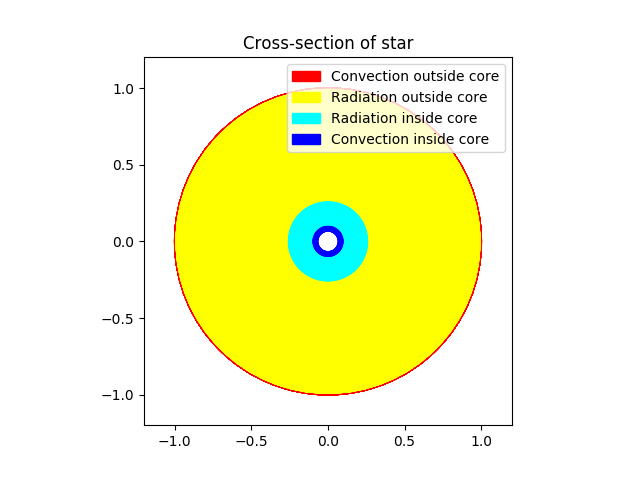
\includegraphics[width = 6cm]{cross_sanity.png}}
\caption{Figures showing the temperature gradients, energy production and the flux.}
\label{fig:nab_eps}
\end{figure}



%https://www.nasa.gov/sites/default/files/images/678410main_layerzoo_full.jpg
%https://sohowww.nascom.nasa.gov/hotshots/index.html/ESA_SOHO_Sun_pgmodes_med.jpg

\begin{thebibliography}{9}

\bibitem{lamport94}
  \textit{Figure \ref{fig:cross}(b)},
  \url{https://soho.nascom.nasa.gov/classroom/images/layers.gif} (downloaded 29.04.18)

\bibitem{2}
  B. V. Gudiksen,
  \textit{AST3310: Astrophysical plasma and stellar interiors},
  \url{http://www.uio.no/studier/emner/matnat/astro/AST3310/v18/beskjeder/notes_v1.pdf} (downloaded 29.04.18)
\end{thebibliography}

\end{document}